% Cyrinx acoustic data-link whitepaper.
% Build: pdflatex cyrinx-acoustic-link.tex (run twice for cross-references).
% All numbers in this document are taken verbatim from the in-repo research
% records: docs/ACOUSTIC_BULK_PHY.md, docs/PRD_VS_AS_BUILT.md,
% scratch/hw20k/NOTES.md, and walkthrough.md (all fresh as of 2026-06-09).
\documentclass[11pt]{article}

\usepackage[letterpaper,margin=1in]{geometry}
\usepackage[T1]{fontenc}
\usepackage[utf8]{inputenc}
\usepackage{microtype}
\usepackage{booktabs}
\usepackage{array}
\usepackage{amsmath}
\usepackage{tikz}
\usepackage{caption}
\usepackage{url}
\usepackage[hidelinks]{hyperref}

\urlstyle{same}
\captionsetup{font=small,labelfont=bf}

\title{\textbf{Cyrinx: A Measured 36.6/27.3\,kbps Bidirectional Acoustic
Data Link Between a Laptop and a Phone}\\[0.5em]
\large An empirical account of building, breaking, and verifying a wideband
OFDM acoustic modem on commodity hardware}

\author{David E. Weekly\thanks{Primatech Paper Co LLC,
\texttt{david@weekly.org}. The modem, diagnostics, and this whitepaper were
developed with substantial AI-agent assistance (Claude Code); all reported
results are from over-the-air measurements on physical hardware recorded in
the project's lab notebook.}}

\date{June 9, 2026}

\begin{document}

\maketitle

\begin{abstract}
We report a software acoustic data link between a MacBook Pro (M4) speaker/microphone
pair and a Google Pixel 7a resting on the laptop's palm rest, achieving
measured, byte-verified over-the-air goodput of \textbf{36{,}571\,bps}
Mac$\rightarrow$Pixel (demodulated \emph{on the phone} by a Kotlin port of the
receiver) and \textbf{27{,}307\,bps} Pixel$\rightarrow$Mac, against a target of
20\,kbps in each direction. Goodput is counted conservatively: only payload
bytes that are both CRC32-valid and byte-identical to the transmitted
pseudorandom sequence, divided by the full airtime span including preambles,
channel-estimation symbols, pilots, FEC redundancy, CRCs, and inter-frame
gaps. The modem is a 48\,kHz OFDM design (FFT 2048, cyclic prefix 768) with
comb pilots, per-symbol timing/phase tracking, uniform 16-QAM, and a punctured
rate-3/4 $K{=}7$ convolutional code. Reaching the target required finding and
fixing four physical-layer defects that are invisible to simulation:
inter-symbol interference from a 10--22\,ms delay spread, decorrelated
dual-speaker transmission, a stream-end fade in the macOS output chain, and
Viterbi poisoning by overconfident log-likelihood ratios from corrupted
symbols. We document the discriminating experiments used to isolate each
defect---including the negative results that exonerated ``obvious''
suspects---and contrast the delivered system with both the original design
document and a predecessor stack whose theoretical 22\,kbps claim corresponded
to a measured 0.27\,kbps. We argue that for acoustic modems on consumer
hardware, the dominant engineering cost is the gap between the channel model
and the channel. None of the modulation or coding machinery here is novel ---
OFDM, cyclic prefixes, comb pilots, QAM, convolutional/Viterbi coding, CRC
block verification, and acoustic data-over-sound are all long established; the
contribution is the \emph{measured} end-to-end system on commodity
heterogeneous hardware, the discriminating-experiment diagnostic methodology,
the physical/platform defect catalog, and on-device verification, not new
modulation theory.
\end{abstract}

\section{Introduction and Motivation}

Consumer laptops and phones ship with speakers and microphones of considerably
higher fidelity than the ``data-over-sound'' literature typically assumes, yet
deployed acoustic-communication systems cluster at very low rates: roughly
$10^2$\,bps for robust spread-spectrum schemes and roughly $10^3$\,bps for
multi-tone FSK \cite{nearby,ggwave}. Acoustic links remain attractive for
proximity-bound exchange---pairing tokens, small payloads, air-gapped
transfer---because sound does not penetrate walls, requires no radio pairing
ritual, and uses hardware already present on billions of devices
\cite{quiet,lisnr}.

The Cyrinx project asked a narrower, harder question: \emph{how much measured
goodput can two specific commodity devices actually exchange acoustically?}
The target was at least 20\,kbps of verified goodput in each direction between
a MacBook Pro (M4) and a Pixel 7a lying face-up on the laptop's palm rest (on
a soft cloth, both devices at maximum volume, normal office ambient noise).
The emphasis on \emph{measured} is deliberate. An earlier in-repo protocol
stack claimed ``22\,kbps'' on the basis of a subcarrier-count capacity formula;
its measured goodput was under 0.3\,kbps (24-byte packets every
$\sim$700\,ms)---a factor of roughly 80 between claim and reality, and a factor
of $\sim$135 between what that stack delivered and what the channel supports
(Section~\ref{sec:eval}). This paper treats that episode as data: every number
reported here is from an over-the-air capture on physical hardware, and we
state explicitly when a figure is an estimate rather than a measurement.

Contributions:
\begin{enumerate}
  \item A characterization of the near-field laptop$\leftrightarrow$phone
        acoustic channel (Section~\ref{sec:channel}): per-band SNR in both
        directions, sample-clock skew, and delay spread.
  \item A wideband OFDM modem design that achieves 36.6/27.3\,kbps verified
        goodput, about 4.5--9$\times$ the original design document's own
        ``optimal conditions'' projection (Section~\ref{sec:design}).
  \item A catalog of four physical-layer defects, each fatal to the link and
        each invisible to simulation, with the discriminating experiments
        (including negative results) that isolated them
        (Section~\ref{sec:defects}).
  \item A verification methodology in which the receiving phone regenerates
        the expected payload locally from a portable deterministic PRNG and
        proves goodput on-device, so no captured samples need leave the phone
        (Section~\ref{sec:detrng}).
\end{enumerate}

\section{Related Work}
\label{sec:related}

The original Cyrinx design document \cite{prd} surveyed the deployed
data-over-sound landscape; we summarize that survey here and credit the
systems directly.

\textbf{libquiet / Quiet Modem Project.} Quiet \cite{quiet,quiethow} brought
soft-decision decoding (via the \texttt{libcorrect} library) to open-source
acoustic networking, with GMSK and PSK modes and Reed--Solomon/convolutional
error correction. Its main limitation is rigidity: the user selects a fixed
profile (e.g.\ \texttt{ultrasonic-experimental} or \texttt{audible-7k}) at
initialization, and there is no feedback loop to adapt constellation density
to the channel. Cyrinx inherits Quiet's conviction that soft decisions matter
--- indeed, our highest-leverage single fix was a soft-decision weighting
refinement (Section~\ref{sec:defects}).

\textbf{minimodem.} A general-purpose FSK/RTTY software modem
\cite{minimodem}. FSK is robust to phase corruption from echoes but spectrally
inefficient, and minimodem deliberately operates as a ``dumb pipe'' with no
integrated FEC \cite{minimodemissue}, delegating integrity to the application.

\textbf{ggwave.} A widely used open-source data-over-sound library using
multi-tone FSK (e.g.\ dividing the spectrum into 96 discrete frequencies and
transmitting 6 tones at once to encode 3 bytes) \cite{ggwave}. Energy-detection
demodulation makes it resilient to multipath, but it does not exploit
high-SNR channels: where QAM can carry 4--6 bits per Hz, MT-FSK carries less
than one.

\textbf{Google Nearby Messages.} The (since deprecated) audio modality of
Nearby used direct-sequence spread spectrum with a 127-chip code, trading
nearly all throughput for detection probability: approximately 94.5\,bps
\cite{nearby,researchgate}. Sufficient for a token, far from bulk transfer.

\textbf{Chirp.io and LISNR.} Commercial closed-source systems
\cite{chirp,lisnr} that emphasized the \emph{wake-up problem}: a cheap,
low-power preamble detector that gates the expensive DSP. LISNR's ``Kilo Audio
Bit'' product claims throughputs around 1\,kbps. Cyrinx adopts the
preamble-gated architecture (a chirp matched filter gates the OFDM decoder)
while being fully open about its error-correction internals.

\textbf{BatNet.} The most directly comparable prior art for a phone-to-phone
ultrasonic link: a smartphone system that carries data between built-in
speakers and microphones using 8-PSK in the 20--24\,kHz inaudible band,
reporting over 600\,bps at up to 6\,m \cite{batnet}. BatNet is the established
demonstration that consumer phone transducers can sustain a coherent
(phase-modulated) ultrasonic link at all; our inaudible-band results
(Section~\ref{sec:future}) are consistent with it on one direction and
illuminate why the other direction fails on the specific Pixel 7a micro-speaker.

\textbf{Synchronization literature.} The predecessor Cyrinx stack used
Zadoff--Chu CAZAC sequences for preamble synchronization and CFO estimation,
following standard practice \cite{cazac,zcfo}, and its robust control-header
modulation (``D-CSS'') was inspired by LoRa-style chirp spread spectrum
\cite{lora}. The bulk PHY described in this paper replaced the ZC preamble
with a linear chirp plus known OFDM sync symbols, and replaced one-shot CFO
estimation with continuous per-symbol pilot tracking---a change forced by
measurement (Section~\ref{sec:defects}).

\textbf{Platform audio stacks.} Prior practitioners documented the hostility
of consumer audio stacks to modem waveforms: voice-processing I/O units inject
echo cancellation and noise suppression that attenuate steady carriers
\cite{vpio,echocancel}, and macOS applies its own processing to chirps
\cite{choi}. Our Android findings (Section~\ref{sec:platform}) are the same
lesson on a different OS: \texttt{AudioSource.UNPROCESSED} is load-bearing,
and the capture path can be silently zeroed by UI state.

Academic work on aerial acoustic communication with consumer hardware
\cite{researchgate} has demonstrated kbps-class links in the near-ultrasonic
band; our contribution is less a novel modulation than a carefully verified
data point---tens of kbps, bidirectional, decoded on the receiving phone---and
a reproducible account of what it took to get there.

\textbf{On originality.} We want to be explicit that the core communications
techniques used here are not original to this work. OFDM, cyclic prefixes,
comb pilots, QAM, punctured convolutional codes with Viterbi decoding, CRC
block verification, acoustic speaker-to-microphone links, and ultrasonic
data-over-sound are all long established, and every system surveyed above
predates and informs ours. We invented no new modulation, code, or
synchronization primitive. The contribution of this paper is instead: (i) a
\emph{measured}, byte-verified end-to-end link on commodity heterogeneous
hardware (a MacBook Pro and a Pixel 7a, decoded on the phone); (ii) a
discriminating-experiment diagnostic methodology, reported with its negative
results; (iii) a catalog of physical-layer and platform defects that are
invisible to simulation; and (iv) on-device verification via a portable
deterministic PRBS. The novelty is empirical and methodological, not
theoretical.

\section{Channel Characterization}
\label{sec:channel}

\subsection{Methodology}

All characterization was over-the-air at the final physical geometry (Pixel 7a
face-up on the MacBook Pro palm rest on a soft cloth). Three probe types were
used, none requiring synchronization between the devices:

\begin{itemize}
  \item \textbf{Probe-on vs.\ probe-off PSD.} A random-phase multitone
        spanning 0.3--23.5\,kHz at digital amplitude 0.6 was played while the
        far device recorded; Welch periodograms (NFFT 1024, 46.875\,Hz bins)
        of probe-on and 6\,s of ambient floor yield per-band SNR without any
        time alignment.
  \item \textbf{Exponential sine sweep (ESS)} for impulse response and delay
        spread.
  \item \textbf{Long pure tone} (10\,kHz, 8\,s) for sample-clock offset, via a
        quadratically interpolated FFT peak.
\end{itemize}

\subsection{Measurements}

Table~\ref{tab:snr} gives the measured SNR by band in both directions
(Mac$\rightarrow$Android, denoted M$\rightarrow$A, uses the Pixel's bottom
microphone, channel 0).

\begin{table}[t]
\centering
\caption{Measured over-the-air SNR by band (Welch PSD, probe-on vs.\ ambient
floor), 2026-06-09. M$\rightarrow$A = Mac speaker to Pixel 7a bottom mic;
A$\rightarrow$M = Pixel speaker to Mac mic.}
\label{tab:snr}
\begin{tabular}{lcc}
\toprule
Band (kHz) & M$\rightarrow$A SNR (dB) & A$\rightarrow$M SNR (dB) \\
\midrule
0.3--2   & 26.4 & 28.1 \\
2--6     & 41.2 & 44.3 \\
6--10    & 37.1 & 47.3 \\
10--14   & 36.0 & 45.5 \\
14--18   & 38.1 & 33.9 \\
18--21   & 36.1 & 10.0 \\
21--24   & 40.7 & \phantom{0}4.6 \\
\bottomrule
\end{tabular}
\end{table}

Key findings, several of which contradicted prior assumptions:

\begin{itemize}
  \item \textbf{The Mac$\rightarrow$Pixel channel is essentially flat to
        23\,kHz} in this near-field geometry. An earlier claim in the project
        history of ``$-32.5$\,dB roll-off at 16\,kHz'' did not reproduce;
        design decisions based on it (a narrow 10--14\,kHz ``flat shelf''
        band) were wrong.
  \item \textbf{The Pixel$\rightarrow$Mac direction dies above
        $\sim$17\,kHz}: 10.0\,dB SNR at 18--21\,kHz falling to 4.6\,dB at
        21--24\,kHz (Pixel speaker and/or Mac microphone roll-off). This
        asymmetry has direct consequences for any inaudible-band variant
        (Section~\ref{sec:future}).
  \item \textbf{Sample-clock offset between the two devices is
        $-24.6$\,ppm}, which at the final OFDM geometry corresponds to about
        0.037 samples of drift per symbol --- small per symbol, but ruinous
        over a frame without continuous tracking.
  \item \textbf{Delay spread (ESS, $-30$\,dB threshold) is $\sim$21.7\,ms
        M$\rightarrow$A and $\sim$10.8\,ms A$\rightarrow$M.} Most energy
        arrives in the first few ms, but the reverberant tail is long; this
        is roughly an order of magnitude larger than the 2\,ms the original
        design document budgeted for.
  \item \textbf{The Pixel's bottom microphone beats its top microphone by
        6--20\,dB below 10\,kHz} at this geometry.
\end{itemize}

From Table~\ref{tab:snr}, Shannon capacity with an 8-bit-per-symbol cap is
approximately 184\,kbps M$\rightarrow$A and 155\,kbps A$\rightarrow$M (an
estimate, not a measurement). The achieved link uses roughly 20--24\% of
that, so substantial headroom remains.

\section{System Design}
\label{sec:design}

\subsection{Modem architecture}

The link is a half-duplex, open-loop bulk-transfer PHY at 48\,kHz PCM16. The
OFDM geometry is NFFT 2048 (23.4\,Hz bins) with a 768-sample cyclic prefix
(16\,ms), giving 17.05 symbols/s; the CP was sized from the measured delay
spread, not from a model. Direction-specific band profiles follow the measured
channel: 1.1--23\,kHz Mac$\rightarrow$Pixel and 0.6--17\,kHz
Pixel$\rightarrow$Mac (Table~\ref{tab:profiles}).

\begin{figure}[t]
\centering
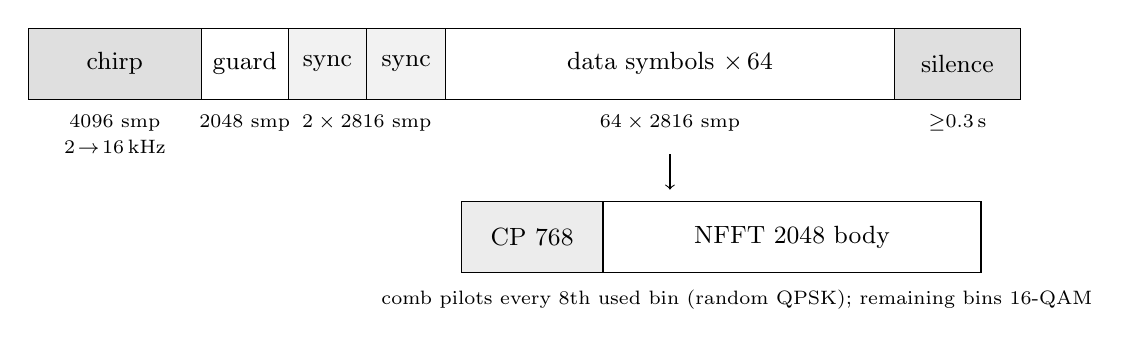
\begin{tikzpicture}[x=1cm,y=1cm,
  blk/.style={draw,minimum height=0.9cm,inner sep=0pt,font=\small},
  lbl/.style={font=\scriptsize}]
 % Frame-level layout (widths not to scale)
 \node[blk,minimum width=2.2cm,fill=gray!25] (chirp) at (1.1,0) {chirp};
 \node[blk,minimum width=1.1cm] (guard) at (2.75,0) {guard};
 \node[blk,minimum width=1.0cm,fill=gray!10] (s0) at (3.8,0) {sync};
 \node[blk,minimum width=1.0cm,fill=gray!10] (s1) at (4.8,0) {sync};
 \node[blk,minimum width=5.7cm] (data) at (8.15,0) {data symbols $\times\,64$};
 \node[blk,minimum width=1.6cm,fill=gray!25] (pad) at (11.8,0) {silence};
 \node[lbl] at (1.1,-0.75)  {4096 smp};
 \node[lbl] at (1.1,-1.05)  {$2\!\to\!16$\,kHz};
 \node[lbl] at (2.75,-0.75) {2048 smp};
 \node[lbl] at (4.3,-0.75)  {$2\times2816$ smp};
 \node[lbl] at (8.15,-0.75) {$64\times2816$ smp};
 \node[lbl] at (11.8,-0.75) {$\geq$0.3\,s};
 % One-symbol inset
 \draw[->,thin] (8.15,-1.15) -- (8.15,-1.6);
 \node[blk,minimum width=1.8cm,fill=gray!15] (cp) at (6.4,-2.2) {CP 768};
 \node[blk,minimum width=4.8cm] (body) at (9.7,-2.2) {NFFT 2048 body};
 \node[lbl,align=left] at (9.0,-3.0)
   {comb pilots every 8th used bin (random QPSK); remaining bins 16-QAM};
\end{tikzpicture}
\caption{Bulk-PHY frame structure (widths not to scale). The chirp gates the
decoder and provides coarse timing; the guard lets the chirp's reverberant
tail decay; two known QPSK sync symbols give the least-squares channel
estimate and a per-bin noise estimate; 64 data symbols follow. The trailing
in-stream silence defends the final symbol against the macOS stream-end fade
(Section~\ref{sec:defects}). One frame spans 192{,}000 samples = 4.0\,s.}
\label{fig:frame}
\end{figure}

Each frame (Figure~\ref{fig:frame}) consists of:

\begin{enumerate}
  \item A 4096-sample linear chirp (2$\to$16\,kHz) for detection and coarse
        synchronization, found by matched filter with threshold-and-suppression
        peak picking for multi-frame runs.
  \item 2048 samples of guard silence so the chirp's reverberation decays
        before channel estimation.
  \item Two known full-band QPSK \emph{sync symbols}. Their average gives a
        per-bin least-squares channel estimate $H$; their difference gives a
        per-bin noise-variance estimate. $H$ is deliberately \emph{not}
        smoothed across bins---under multipath its phase rotates through
        multiple cycles across a few bins and smoothing destroys it (only the
        real, positive noise variance is smoothed).
  \item 64 data symbols. Every 8th used bin carries a comb pilot (random
        QPSK); the rest carry uniform 16-QAM. Per symbol, a three-pass
        iterative fit of the pilot phase ramp extracts a timing slope plus
        common phase error and corrects all bins, absorbing the $-24.6$\,ppm
        clock skew continuously. (Per-bin adaptive loading is implemented but
        was not needed to reach the target.)
\end{enumerate}

FEC is a $K{=}7$ (171,133) convolutional code, punctured to rate 3/4
(pattern 110110), zero-terminated, with soft max-log LLRs, a frame-wide
pseudorandom interleaver, and Viterbi decoding. Payload is segmented into
256-byte blocks, each with a CRC32, purely for honest goodput accounting.
Two further measured-channel adaptations are part of the transmit contract:
the FFT window is biased 24 samples early so multipath pre-cursors stay inside
the CP, and Mac$\rightarrow$Pixel transmission uses the \emph{left speaker
only} (Section~\ref{sec:defects}).

The load-bearing receiver refinement is \textbf{per-symbol LLR weighting}:
each data bin's noise variance is taken as the sync-derived per-bin estimate
\emph{plus that symbol's own pilot error-vector magnitude squared}. A symbol
corrupted by a burst, dropout, or fade therefore reports honestly weak LLRs
and degrades into soft erasures rather than poisoning the Viterbi traceback
through the interleaver (Section~\ref{sec:defects}, defect 4). This also
provides burst-noise immunity (typing, key clicks) at no added cost.

\begin{table}[t]
\centering
\caption{Direction-specific transmit profiles (16-QAM, rate 3/4, 64 data
symbols/frame). Bin counts and per-frame payload follow from the band edges
and the 23.4\,Hz bin spacing.}
\label{tab:profiles}
\begin{tabular}{lcc}
\toprule
 & Mac$\rightarrow$Pixel & Pixel$\rightarrow$Mac \\
\midrule
Band & 1.1--23\,kHz & 0.6--17\,kHz \\
Used bins & 935 & 700 \\
~~of which pilots & 117 & 88 \\
~~of which data (16-QAM) & 818 & 612 \\
Coded bits/symbol & 3272 & 2448 \\
CRC32 blocks/frame & 75 & 56 \\
Payload/frame & 19{,}200\,B & 14{,}336\,B \\
Frame airtime & 4.0\,s & 4.0\,s \\
Transmit quirk & left speaker only & --- \\
\bottomrule
\end{tabular}
\end{table}

\subsection{Portable deterministic streams and on-device verification}
\label{sec:detrng}

All deterministic streams in the modem---pilot phases, sync symbols, the
interleaver permutation, payload-padding bits, and the test payload itself---
derive from a shared \texttt{splitmix64} generator (\texttt{DetRng}),
implemented identically in Python (\texttt{scratch/hw20k/modem.py}) and Kotlin
(\texttt{BulkDemod.kt}). This small trick has an outsized methodological
payoff: the phone regenerates the \emph{expected} payload bytes locally from
the seed and compares them against what it decoded, so end-to-end goodput is
proven on the receiving device itself and no captured audio or decoded data
needs to leave the phone. The Kotlin receiver is a port of the Python receive
path (including a double-precision radix-2 FFT written for the purpose) and
was validated bit-compatible against the Python decoder on an identical
capture file (225/225 blocks, matching EVM) before the live runs.

\subsection{What the bulk PHY deliberately omits}

Relative to the original design document \cite{prd}, the bulk PHY drops the
per-frame TDD ping-pong MAC with ACK/channel-state reports, rateless
(Raptor/LDPC) coding, and the rate-adaptation ``gear'' state machine. The
predecessor stack implemented that chatty MAC, and its turnaround gaps, tiny
payloads, and ACK timeouts consumed more than 97\% of airtime---this is why it
measured 0.27\,kbps. For bulk transfer, long streaming frames with open-loop
MCS selection from the measured channel are the right shape; closed-loop
adaptation belongs at session granularity, not frame granularity. Encryption
(an X25519/CTR/HMAC envelope exists in the predecessor stack), discovery, and
ARQ are likewise out of scope for the PHY measurement reported here.

\section{What Didn't Work: Four Defects and the Experiments That Found Them}
\label{sec:defects}

The first end-to-end attempts decoded zero blocks despite a channel with
35--45\,dB of mid-band SNR. Four distinct physical-layer defects were stacked
on top of each other; each was fatal alone, and none is visible in a
simulation. All were diagnosed on real captures. We describe them in
discovery order, then the diagnostic method.

\subsection{The defects}

\textbf{Defect 1: ISI --- delay spread far exceeds the cyclic prefix.}
The initial geometry (NFFT 1024, CP 256 = 5.3\,ms) assumed a short channel.
A repeated-symbol probe showed adjacent \emph{identical} symbols agreeing at
24--27\,dB while adjacent \emph{different-content} symbols agreed at only
11--13\,dB --- the signature of inter-symbol interference, not noise or
channel instability. The geometry moved to NFFT 2048 / CP 768 (16\,ms),
consistent with the measured 10--22\,ms delay spread.

\textbf{Defect 2: dual-speaker transmission corrupts the composite.}
With the phone on the left palm rest, the right speaker's signal arrives about
3$\times$ weaker with decorrelated phase (EVM 1.33 received alone); summed
with the left speaker it drags composite EVM to $\sim$0.5. Transmitting from
the left speaker only gives EVM $\sim$0.06. (A true 2$\times$2 MIMO receiver
with per-stream equalization could exploit the second speaker; it was not
needed to reach the target.)

\textbf{Defect 3: stream-end fade kills the final symbol.}
The macOS speaker chain tapers the last $\sim$10\,ms when an output stream
stops. Per-symbol raw BER against the known coded stream was 0.000 for
symbols 0--14 and 0.264 for the final symbol. With a frame-wide interleaver,
that one dead symbol contaminates \emph{every} FEC block. Fix: at least 0.3\,s
of trailing silence inside the stream, so the fade lands on padding.

\textbf{Defect 4: overconfident LLRs from a corrupted symbol poison Viterbi.}
Even one corrupted symbol in 16 ($\approx$1.7\% average raw BER, trivially
correctable in principle) yielded only 0--1 of 6 blocks, because the corrupted
symbol's wrong LLRs carried full confidence through the interleaver into the
Viterbi metric. Weighting each symbol's LLRs by its own pilot EVM$^2$ turns
such symbols into soft erasures; the same captured regression then decodes
6/6. This was the single highest-leverage coding change in the project.

\subsection{Diagnostic methodology, including negative results}

The defects above were separated by discriminating experiments, several of
which mattered precisely because they \emph{exonerated} a suspect. We list
them as first-class results; all are reusable scripts in
\texttt{scratch/hw20k/}.

\begin{itemize}
  \item \textbf{Repeated-symbol probe.} Transmit $N$ identical OFDM symbols.
        Identical-vs-different-content consistency separates ISI from channel
        instability, dropped samples, and clock drift; the phase trace across
        repeats measured drift cleanly (linear in time, proportional to
        frequency $\Rightarrow$ pure clock skew, channel stable).
  \item \textbf{Amplitude ladder} (digital amplitude 0.07$\to$0.7): EVM was
        flat across 20\,dB of drive level, \emph{exonerating} speaker
        nonlinearity and speaker-protection DSP as the dominant impairment ---
        despite being the ``obvious'' suspect at maximum volume.
  \item \textbf{\texttt{afplay} vs.\ \texttt{sounddevice} A/B} on the
        identical frame file: identical EVM, \emph{exonerating} the playback
        software path.
  \item \textbf{Genie TX/RX ratio test.} FFT the saved transmit waveform and
        the capture at matching symbol positions and compare directly:
        adjacent-symbol consistency held at 15\,dB while sync-to-late-symbol
        agreement degraded smoothly --- the channel was fine; the receiver's
        tracking was at fault.
  \item \textbf{Piecewise TX$\leftrightarrow$RX alignment.} Correlating
        successive transmit chunks against the capture detects dropped
        samples (none found; a smooth $+24$\,ppm drift instead) and revealed
        the correlator tap-hopping between two multipath arrivals $\sim$19
        samples apart --- motivating the 24-sample-early window bias.
  \item \textbf{Per-symbol raw BER} against the known coded stream localized
        failure to exactly the final symbol (defect 3) when aggregate metrics
        (EVM, mean BER) merely looked ``mediocre.''
\end{itemize}

\textbf{A cautionary tale about debug tooling.} An early debug script mixed
module-level FFT/CP constants with a differently configured modem object and
fabricated a ``0\,dB sync consistency'' reading that misdirected the
investigation for a full round. The lesson is procedural: diagnostic tooling
must share the \emph{exact} configuration object with the system under test.
The script survives in the repo, fixed and carrying a warning comment, as a
reminder.

\section{Evaluation}
\label{sec:eval}

\subsection{Stepped modulation results}

With all four defects fixed, modulation and code rate were stepped upward on
real over-the-air captures (offline decode; 5-frame runs; goodput includes all
overhead and 0.25\,s inter-frame gaps). Table~\ref{tab:steps} shows clean
decodes at every step; both directions cross the 20\,kbps target at 16-QAM
rate 3/4.

\begin{table}[t]
\centering
\caption{Stepped over-the-air results (offline decode of real captures,
2026-06-09). All blocks CRC-valid at every step.}
\label{tab:steps}
\begin{tabular}{llccc}
\toprule
Direction & Profile & Blocks & EVM & Goodput \\
\midrule
M$\rightarrow$A (1.1--23\,kHz) & QPSK r1/2  & 75/75   & 0.06 & 12.29\,kbps \\
M$\rightarrow$A & 16-QAM r1/2 & 150/150 & 0.06 & 24.58\,kbps \\
M$\rightarrow$A & 16-QAM r3/4 & 225/225 & 0.07 & \textbf{36.86\,kbps} \\
\midrule
A$\rightarrow$M (0.6--17\,kHz) & QPSK r1/2  & 54/54   & 0.12 & \phantom{0}8.85\,kbps \\
A$\rightarrow$M & 16-QAM r1/2 & 111/111 & 0.12 & 18.19\,kbps \\
A$\rightarrow$M & 16-QAM r3/4 & 168/168 & 0.11 & \textbf{27.53\,kbps} \\
\bottomrule
\end{tabular}
\end{table}

\subsection{Final verified measurement}

The definitive run (\texttt{scratch/hw20k/final\_measurement.py}) transmits
5 frames per direction at 16-QAM rate 3/4 and counts goodput as payload bytes
that are both CRC32-valid \emph{and} byte-identical to the transmitted
\texttt{DetRng} PRBS, divided by the span from the first frame's chirp to the
last frame's final data sample --- preambles, sync symbols, pilots, FEC
redundancy, CRCs, and inter-frame gaps all count against the number. Each
direction spans 21.0\,s of airtime.

\begin{table}[t]
\centering
\caption{Final byte-verified over-the-air goodput (2026-06-09). The
Mac$\rightarrow$Pixel capture was demodulated and verified on the Pixel
itself; it never left the phone.}
\label{tab:final}
\begin{tabular}{llcc}
\toprule
Direction & Decoder & Blocks verified & Goodput \\
\midrule
Mac$\rightarrow$Pixel 7a (1.1--23\,kHz) & on the Pixel (\texttt{BulkDemod.kt}) &
  375/375 (96{,}000\,B) & \textbf{36{,}571\,bps} \\
Pixel 7a$\rightarrow$Mac (0.6--17\,kHz) & on the Mac (\texttt{modem.py}) &
  280/280 (71{,}680\,B) & \textbf{27{,}307\,bps} \\
\bottomrule
\end{tabular}
\end{table}

Both directions exceed the 20\,kbps goal with zero block errors
(Table~\ref{tab:final}). The on-device Kotlin decoder runs in about 170\,ms
per 4\,s frame on the Pixel 7a --- roughly 20$\times$ real time --- in pure
Kotlin with a double-precision radix-2 FFT, which indicates that a real-time
streaming receiver is computationally comfortable on this class of phone.

\subsection{Contrast with the predecessor stack}

The predecessor in-repo stack (Zadoff--Chu sync, D-CSS headers, OFDM-QPSK
payload, per-frame ACK MAC) reported a ``symmetrical 20+\,kbps'' result that
was, on inspection, a capacity formula ($86$ carriers $\times$ 6 bits $\times$
42.857 symbols/s $=22.11$\,kbps); its measured goodput was under 0.3\,kbps.
The project history now carries a correction notice. The channel supported
roughly 135$\times$ what that stack delivered; the loss was architectural
(turnaround gaps, 24-byte payloads, ACK timeouts) rather than physical. We
include this not to disparage the earlier effort --- its Kotlin FFT,
HIL tooling, and platform groundwork carried forward --- but because the
simulation-vs-measurement gap is the central finding of the project.

\section{Platform Findings}
\label{sec:platform}

Two classes of platform behavior materially affected measurement integrity
and are worth recording for other practitioners.

\textbf{Android silently records zeros when the activity is not top-visible.}
A secure-lockscreen bouncer (\texttt{AlternateBouncerView}) or an expanded
notification shade both trigger the audio policy's capture silencing
(\texttt{dumpsys audio} shows the record client as \texttt{silenced}); the
capture API succeeds and returns buffers of zeros. Mitigations:
\texttt{setShowWhenLocked(true)} and \texttt{setTurnScreenOn(true)} on the
activity, collapsing the status bar (\texttt{cmd statusbar collapse}), and a
wake sequence before every capture. Battery saver at low charge re-dozes the
screen despite \texttt{svc power stayon}. Separately,
\texttt{AudioRecord} with \texttt{AudioSource.UNPROCESSED} at 48\,kHz stereo
works on the Pixel 7a and is mandatory: processed sources apply AGC and noise
suppression that would corrupt QAM phase.

\textbf{macOS gotchas.} The Mac microphone clips near-field at full input
volume (captures rail at $\pm$1.0); input volume around 22/100 is appropriate
for a phone speaker at maximum on the palm rest. The native 48\,kHz devices
must be selected explicitly --- external displays and Bluetooth headsets
silently become the default device and hijack playback. And, as defect 3
showed, the output chain's stream-end fade is part of the channel.

\section{Limitations and Future Directions}
\label{sec:future}

\textbf{Limitations of the result as it stands.} These are scope statements,
not failures; we state them plainly so the result is not over-read. The
measured bulk PHY: (i) is \emph{not} integrated into the project's public
Swift/C transport API --- it lives in the research harness
(\texttt{scratch/hw20k/}) and the Kotlin HIL decoder; (ii) is \emph{not}
real-time streaming --- it is a batch design that records, then decodes
offline, though the on-device decoder runs at roughly 20$\times$ real time and
a streaming port is therefore plausible; (iii) is \emph{not} closed-loop
rate-adaptive --- the MCS is chosen open-loop from a same-day channel
measurement, with no per-frame feedback; (iv) is \emph{not} secured by the
project's existing X25519/CTR/HMAC envelope --- the PHY measurement carries
raw test payloads; and (v) is validated in exactly \emph{one} physical
geometry (a Pixel 7a face-up on a MacBook Pro palm rest), on one device pair,
under one ambient condition. The link is half-duplex and has no link layer.
The numbers should be read as ``what this hardware pair can do at contact
range,'' not as a general-environment claim.

\textbf{Untapped physical headroom} (estimates, from the measured SNR):
\begin{itemize}
  \item \emph{Per-bin adaptive bit loading.} Mid-band SNR is 35--45\,dB;
        64/256-QAM there should roughly double throughput. The loading
        machinery already exists in the modem.
  \item \emph{Maximal-ratio combining} of the Pixel's two microphones
        (the bottom mic leads the top by 6--20\,dB below 10\,kHz; MRC adds
        diversity above).
  \item \emph{True 2$\times$2 MIMO} (Mac stereo speakers $\times$ Pixel
        stereo mics) for spatial multiplexing Mac$\rightarrow$Pixel ---
        turning defect 2's decorrelation from a bug into capacity.
  \item \emph{Real-time streaming RX.} At 20$\times$ real time for the batch
        decoder, a ring-buffer port is straightforward.
  \item \emph{Link layer:} session-granularity rate adaptation from
        receiver-fed-back per-bin SNR, plus ARQ for residual block errors at
        higher MCS.
\end{itemize}

\subsection{Measured result: the inaudible-ultrasonic variant}
\label{sec:ultrasonic}

The original goal (and the obvious product form) is an inaudible link in the
18.5--23.9\,kHz band. We subsequently ran the bulk-PHY methodology entirely in
that band at 96\,kHz sampling \cite{ultrasonicband}; the answer is that it is
\emph{feasible in one direction but transducer-bound in the other}.

\textbf{Mac$\rightarrow$Pixel works.} In the 18.5--23.9\,kHz band at 96\,kHz
(NFFT 2048, CP 768, the chirp preamble moved up into 18.6--23.4\,kHz),
16-QAM rate 3/4 delivers \textbf{$\sim$9\,kbps} of verified goodput at
EVM $\sim$0.11, with every block recovered. The ceiling here is bandwidth, not
modulation: a $\sim$5.4\,kHz coherent band at $\sim$22\,dB SNR caps near
9--10\,kbps, and reaching 20\,kbps inaudibly would require either more coherent
ultrasonic bandwidth than this Pixel offers or dropping below 18.5\,kHz
(audible).

\textbf{Pixel$\rightarrow$Mac does not close} --- and the reason is a clean
physical result rather than a tuning failure. The Pixel 7a micro-speaker is
\emph{phase-incoherent} above $\sim$18\,kHz: a single-tone STFT phase-jitter
measurement gives a detrended phase standard deviation of 0.055\,rad at 8\,kHz
(clean) versus 2--4\,rad at 19.5--22\,kHz (incoherent at the upper end). The
speaker radiates ultrasonic \emph{power}, but cannot reproduce it with the
phase coherence that OFDM/QAM --- or any phase modulation --- requires. This
resolves an apparent contradiction in the channel survey: a stationary
multitone PSD reports $\sim$27.8\,dB ``SNR'' for Pixel$\rightarrow$Mac at
18.5--21\,kHz, yet coherent OFDM demodulation in the same band yields
EVM $\sim$1.0 (SINR $\sim$0\,dB). Power-per-bin and phase coherence are
different quantities; PSD-based channel surveys overstate capacity for
phase-modulated waveforms on this transducer. A room-tone capture confirmed
the band is near-silent (in-band RMS $\sim$5$\times$10$^{-8}$), so the limit is
the transmit transducer, not ambient noise.

The conclusion is that a \emph{symmetric} inaudible link is bounded by the
mobile speaker, not by the protocol. The fast inaudible direction
(Mac$\rightarrow$Pixel, $\sim$9\,kbps) is real; the inaudible return path would
require a non-coherent modulation (energy-based MFSK or OOK, as ggwave uses)
to tolerate the micro-speaker's phase incoherence, at much lower rates.

\section{Summary of Findings}

\begin{enumerate}
  \item A laptop and a phone at contact range can exchange tens of kbps
        acoustically: \textbf{36{,}571\,bps} Mac$\rightarrow$Pixel 7a and
        \textbf{27{,}307\,bps} Pixel$\rightarrow$Mac, byte-verified, with all
        overhead counted --- roughly two orders of magnitude above deployed
        data-over-sound systems, and 4.5--9$\times$ the project's own design
        document projection. The headline enabler was abandoning the
        inaudibility constraint, which widened the channel from 5\,kHz to
        16--22\,kHz.
  \item The measured channel, not the modeled one, dictated every major
        design parameter: CP length (delay spread is $\sim$10$\times$ the
        modeled value), pilot structure (clock skew, not Doppler, is the
        always-present phase enemy), speaker selection, and band edges
        (Pixel$\rightarrow$Mac dies above 17\,kHz).
  \item Four stacked, simulation-invisible defects each individually killed
        the link; cheap discriminating experiments --- including negative
        results that exonerated nonlinearity and the playback path ---
        isolated them. Per-symbol pilot-EVM LLR weighting (soft erasures) was
        the highest-leverage single fix.
  \item Verification discipline matters: a deterministic cross-language PRBS
        lets the receiving phone prove goodput on-device, and a conservative
        goodput definition (verified bytes over total airtime) keeps the
        result honest. The predecessor stack's 80$\times$ claim-to-measurement
        gap is the cautionary baseline.
  \item Consumer audio platforms are an active part of the channel: Android
        silently zeroes capture based on UI visibility, processed capture
        paths corrupt QAM, and macOS fades stream tails. Budget for the OS.
\end{enumerate}

\begin{thebibliography}{99}
\small

\bibitem{quiet}
Quiet Modem Project. ``Quiet.'' \url{https://quiet.github.io/}
(accessed February 12, 2026).

\bibitem{quiethow}
Quiet Modem Project. ``How It Works.''
\url{https://quiet.github.io/docs/org.quietmodem.Quiet/how/}
(accessed February 12, 2026).

\bibitem{researchgate}
``Ultrasonic Communication Using Consumer Hardware.''
\url{https://www.researchgate.net/publication/320575022_Ultrasonic_Communication_Using_Consumer_Hardware}
(accessed February 12, 2026).

\bibitem{nearby}
Google for Developers. ``Get Started --- Nearby Messages API for Android.''
\url{https://developers.google.com/nearby/messages/android/get-started}
(accessed February 12, 2026).

\bibitem{minimodem}
``minimodem --- general-purpose software audio FSK modem.'' Ubuntu manpage.
\url{https://manpages.ubuntu.com/manpages/xenial/man1/minimodem.1.html}
(accessed February 12, 2026).

\bibitem{minimodemissue}
kamalmostafa/minimodem, GitHub issue \#30 (on the absence of integrated FEC).
\url{https://github.com/kamalmostafa/minimodem/issues/30}
(accessed February 12, 2026).

\bibitem{ggwave}
G.~Gerganov. ``ggwave: Tiny data-over-sound library.''
\url{https://github.com/ggerganov/ggwave} (accessed February 12, 2026).

\bibitem{batnet}
A.~Zarandy, I.~Shumailov, R.~Anderson. ``BatNet: Data transmission between
smartphones over ultrasound.'' arXiv:2008.00136, August 2020.
\url{https://arxiv.org/abs/2008.00136} (accessed June 9, 2026).

\bibitem{chirp}
InvenSense (TDK). ``AN-000225: Ultrasonic range sensing enables measured
social contact'' (Chirp white paper).
\url{https://invensense.tdk.com/wp-content/uploads/2020/08/AN-000225-Chirp-Social-Distancing-White-Paper-v1.0_8_3_20-2.pdf}
(accessed February 12, 2026).

\bibitem{lisnr}
LISNR. ``How Does Data over Audio Transmission Work?''
\url{https://lisnr.com/resources/blog/data-over-audio-transmission/}
(accessed February 12, 2026).

\bibitem{cazac}
``Timing and Frequency Synchronization Using CAZAC Sequences.'' MDPI.
\url{https://www.mdpi.com/1424-8220/23/6/3168} (accessed February 12, 2026).

\bibitem{zcfo}
``Analysis of the Frequency Offset Effect on Zadoff--Chu Sequence Timing
Performance.'' arXiv. \url{https://arxiv.org/pdf/1406.3412}
(accessed February 12, 2026).

\bibitem{lora}
Semtech Corporation. ``AN1200.22: LoRa Modulation Basics.'' Application note.

\bibitem{vpio}
``VoiceProcessingIO Audio Unit adds an unexpected input stream to Built-in
output device (macOS).'' Stack Overflow.
\url{https://stackoverflow.com/questions/64966350/voiceprocessingio-audio-unit-adds-an-unexpected-input-stream-to-built-in-output}
(accessed February 12, 2026).

\bibitem{echocancel}
Apple Developer Documentation. ``setPrefersEchoCancelledInput(\_:).''
\url{https://developer.apple.com/documentation/avfaudio/avaudiosession/setprefersechocancelledinput(_:)}
(accessed February 12, 2026).

\bibitem{choi}
H.~Choi. ``Audio chirp processing problems on OS X.''
\url{http://henryomd.blogspot.com/2017/03/audio-chirp-processing-problems-on-os-x.html}
(accessed February 12, 2026).

\bibitem{iphonemic}
Faber Acoustical. ``Measured: iPhone 15 Pro Max microphone frequency response
and directivity.''
\url{https://blog.faberacoustical.com/wpblog/2024/ios/iphone/measured-iphone-15-pro-max-microphone-frequency-response-and-directivity/}
(accessed February 12, 2026).

\bibitem{applerates}
Apple Support. ``Play high sample rate audio on your Mac.''
\url{https://support.apple.com/en-us/108326} (accessed February 12, 2026).

\bibitem{prd}
``Cyrinx: A High-Fidelity Adaptive Ultrasonic Transport Protocol ---
Technical Product Requirements Document \& Research Report,'' February 2026.
Internal design document; contrasted with the as-built system in
\texttt{docs/PRD\_VS\_AS\_BUILT.md} of the Cyrinx repository.

\bibitem{ultrasonicband}
``Ultrasonic-Band (Inaudible) Bulk PHY --- Measured Results,''
\texttt{docs/ULTRASONIC\_BAND.md} of the Cyrinx repository, June 2026.
Fresh as of 2026-06-09.

\bibitem{repo}
Cyrinx repository research records: \texttt{docs/ACOUSTIC\_BULK\_PHY.md}
(research writeup), \texttt{scratch/hw20k/NOTES.md} (lab notebook),
\texttt{scratch/hw20k/} (modem, harness, and diagnostic scripts), and
\texttt{Apps/HIL/android/.../BulkDemod.kt} (on-device Kotlin decoder).
All fresh as of 2026-06-09.

\end{thebibliography}

\end{document}
